\documentclass{article}
\usepackage{amsmath}
\usepackage{optidef}
\usepackage{amssymb}
\usepackage[utf8x]{inputenc}
\usepackage{graphicx}
\usepackage[]{algorithm2e}
\graphicspath{ {rsc/} }
\allowdisplaybreaks
\title{Rapport technique}
\author{
	AUGUSTO Rold 
	\and 
	PAUL Hugo 
	\and 
	TRANG Hoang Phong Vu
	\and 
	SUGANATHASIVAM Vathanalakshan
	}
	
\begin{document}
\maketitle
\section{Intoduction}
TODO : Introduction
\section{Problème du voyageur de commerce déterministe}
Afin de pouvoir traiter le problème du voyageur de commerce stochastique, nous partons de l'origine avec une approche déterministe. Dans cette approche, les distances entre les villes sont connues avant que le commerçant commence le voyage.  Plus concrètement, soit:\\
\begin{itemize}
\item G = (V, E) un graphe orienté ou non-orienté complet avec :
		\begin{itemize}
			\item V l'ensemble de sommets
			\item \( E \subseteq \{(x, y) | (x, y) \in V^2 \wedge x \neq y \} \) l'ensemble d'arêtes
		\end{itemize}
\item \(c_{ij}\) le coût pour aller du sommet \(v_{i}\) au sommet \(v_{j}\)
\item \(x_{ij}\) la variable de décision. elle vaut 1 s'il existe un arc \((v_{i}, v_{j})\), 0 sinon. On peut l'interpréter comme une matrice de passage.
\end{itemize}
Le problème du voyageur de commerce peut être écrit sous forme mathématique suivant :
\begin{mini!}|s|[1]                   % mini! = minimize 
    {x}                               % optimization variable
    {\sum_{i=1}^{n}\sum_{j=1}^{n}c_{ij}x_{ij}\label{eq:optd}}   % objective function and label
    {\label{eq:Example1}}             % label for optimization problem
    {}                                % optimization result
    \addConstraint{\sum_{j=1, i \neq j}^{n} x_{ij}}{= 1, \quad & i = 1,...  \label{eq:optd_con1}}
    \addConstraint{\sum_{i=1, i \neq j}^{n} x_{ij}}{= 1, \quad & j = 1,...  \label{eq:optd_con2}}   
    \addConstraint{\sum_{i|v_i \in S} \sum_{j|v_j \in S}x_{ij}} {\leq |S| - 1 \quad & S \subset V \textrm{et} S \neq \varnothing \label{eq:optd_con3}}
    \addConstraint{x_{ij} } {\in \{0, 1\} \quad & 1 \leq i, j \leq n \label{eq:optd_con4}}
\end{mini!}
D'une manière littérale, le voyageur doit visiter toutes les villes (connues dans le graphe) tel que la distance qu'il parcourt est minimale et que pour chaque ville il ne peut visiter qu'une seule fois. Plus concrètement, la fonction objectif sert à trouver la distance minimale. La contrainte \ref{eq:optd_con1} veut dire : après avoir visté une ville \(v_i\), le voyageur ne peut visiter qu'une ville ensuite. Avec la contrainte \ref{eq:optd_con2}, lors d'une visite d'une ville \(v_j\), le voyageur ne peut provenir que d'une seule ville.\\
En comparant avec les conditions littérales que nous avons prises en compte précédémment, les deux premières contraintes sont suffisantes. Néanmoins, les algorithmes d'optimisation des solveurs peuvent génerer des subtours (i.e. sous chemins). Le fait d'avoir plusieurs chemins discrètes veut dire que le voyageur a le droit de sauter d'une ville en une autre ville sans prendre en compte la distance parcourue et ce n'est pas logique. La contrainte (\ref{eq:optd_con3}) est donc rajoutée au modèle pour les éliminer, elle est appelée la contrainte d'élimination des subtours.\\

\begin{figure}[h]\centering
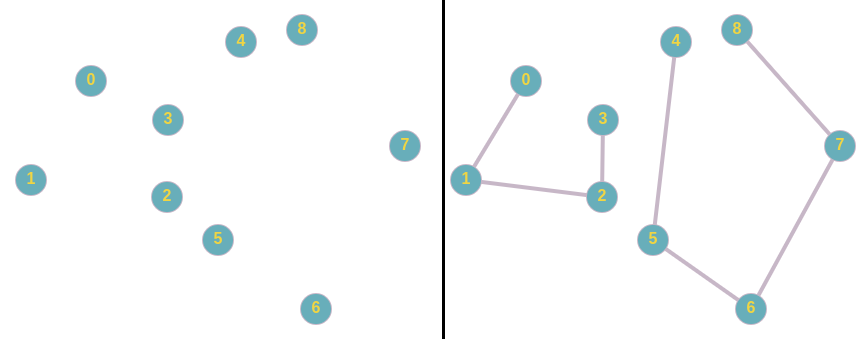
\includegraphics[width=0.5\textwidth]{graphe_avec_subtour}
\caption{Une solution où existe plusieurs subtours (sous-chemins) (Attention, il s'agit d'un exemple pour montrer la conséquence d'une manque de la contrainte \ref{eq:optd_con4}, elle n'est donc pas une solution optimale)}

\end{figure}
Une approche possible pour ce modèle est de lancer l'optimisation avec les contraintes (\ref{eq:optd_con1}), (\ref{eq:optd_con2}), (\ref{eq:optd_con4}) plusieurs fois jusqu'à ce qu'on obtient la solution optimale. La démarche est exprimée dans le pseudo-code ci-dessous :\\
\begin{algorithm}[H] 
 \KwData{graphe G=(V, E)}
 \KwResult{La solution optimale du problème du voyageur de commerce}
   nS \(\leftarrow +\infty\)  \;
 \While{nS n'est pas optimale}{
  lancer l'optimisation avec les contraintes \ref{eq:optd_con1} \ref{eq:optd_con2} \ref{eq:optd_con4}\;
  nS \(\leftarrow\) nombre de sous graphes de l'optimisation\;
 }
 \caption{Trouver la solution optimale du problème du voyageur de commerce}
\end{algorithm}
En effet, pour la contrainte d'élimination de subtours, il existe plusieures formulations possibles. Dans le cadre de notre projet, on a décidé d'utiliser celle de Miller-Tucker-Zemlin pour des raisons de simplicité et efficacité:
\begin{equation}
\begin{aligned}
	u_i - u_j + nx_{ij} \leq n - 1, \quad & 2 \leq i \neq j \leq n \\
	1 \leq u_j \leq n - 1, \quad & 2 \leq i \leq n
\end{aligned}
\end{equation}
La variable \(u_i \in \mathbb{N} \cup \{0\}\) est une variable de décision, elle indique l'ordre de passage de la ville i. De ce fait, \(u_i \leq u_j\) implique que la ville i est visité avant la ville j.\\

\section{Problème du voyageur de commerce stochastique}
Nous avons traité le problème du voyageur de commerce de façon exacte où les coûts (i.e les distance, la durée, etc.) sont connus dans la partie précédente. En réalité, le voyageur peut rencontrer les difficultés survenues telles que des travaux, le blocage de la circulation, etc. Dans ces cas là, il doit changer les routes pour pouvoir continuer son voyage. Nous allons modéliser cette contrainte dans la suite de la partie. Pour cela, on considère que les coûts \(\tilde{c}\)  ne sont plus exacts mais des variables aléatoires. Ils suivent la distribution normale dont la moyenne est \(\bar{c}\) et la matrice de variance-covariance est \(\sum\) : \(\tilde{c_{ij}} \sim \mathcal{N}(\bar{c_{ij}},\,\sigma_{ij}^{2})\, \). En effet, On veut que la distance en réalité soit au tour de la distance théorique, la moyenne \(\bar{c_{ij}}\) ci-dessus est donc celle du problème déterministe \(c_{ij}\) (la distance théorique).\\
Le modèle mathématique devient donc :
\begin{mini!}|s|[2]                   % mini! = minimize 
    {x}                               % optimization variable
    {\sum_{i=1}^{n}\sum_{j=1}^{n}\bar{c_{ij}}x_{ij}\label{eq:opts}}   % objective function and label
    {\label{eq:Example1}}             % label for optimization problem
    {}                                % optimization result
    \addConstraint{\sum_{j=1, i \neq j}^{n} x_{ij}}{= 1, \quad & i = 1,...  \label{eq:opts_con1}}
    \addConstraint{\sum_{i=1, i \neq j}^{n} x_{ij}}{= 1, \quad & j = 1,...  \label{eq:opts_con2}}   
    \addConstraint{\sum_{i|v_i \in S} \sum_{j|v_j \in S}x_{ij}} {\leq |S| - 1 \quad & S \subset V \textrm{et} S \neq \varnothing \label{eq:opts_con3}}
    \addConstraint{P ( \sum_{i=1}^{n}\sum_{j=1}^{n}\tilde{c_{ij}}x_{ij} \leq Z) \geq \alpha \label{eq:opts_con4}}
    \addConstraint{x_{ij} } {\in \{0, 1\} \quad & 1 \leq i, j \leq n \label{eq:opts_con5}}
\end{mini!}
La contrainte (\ref{eq:opts_con4}) a été rajoutée dans ce modèle. Elle est appelée contrainte en probabilité ou la contrainte stochastique. Elle modélise le risque pris par le voyageur de commerce, et doit être satisfaite dans au moins de \(\alpha\%\) des cas. La constante Z est la valeur de la solution optimale du problème déterministe majorée de 20 à 30\%.\\
On peut voir que ce n'est pas possible d'implémenter directement la contrainte en probabilité (\ref{eq:opts_con4}) en CPLEX. Il faut donc transformer la probabilité en une autre forme.\\
Plus concrètement:\\
\begin{equation}
\begin{aligned}
\textrm{On a : } 
& \tilde{c_{ij}} \sim \mathcal{N}(\bar{c_{ij}},\,\sigma_{ij}^{2})\\
&\Rightarrow x_{ij}\tilde{c_{ij}} \sim \mathcal{N}(x_{ij}\bar{c_{ij}},\, x_{ij}^2\sigma_{ij}^{2})\\
&\Rightarrow \sum_{i}^n \sum_{j}^n x_{ij}\tilde{c_{ij}} \sim \mathcal{N}(\sum_{i}^n \sum_{j}^n x_{ij}\bar{c_{ij}},\, \sum_{i}^n \sum_{j}^n x_{ij}^2\sigma_{ij}^{2})\\
&\textrm{Appelons } X = \sum_{i}^n \sum_{j}^n x_{ij}\tilde{c_{ij}}\\ 
&\Rightarrow X \sim \mathcal{N}(\sum_{i}^n \sum_{j}^n x_{ij}\bar{c_{ij}},\, \sum_{i}^n \sum_{j}^n x_{ij}^2\sigma_{ij}^{2})\\
\textrm{(\ref{eq:opts_con4}) devient :} 
& P(X \leq Z) \geq \alpha \\
&\Leftrightarrow F_X(Z) \geq \alpha\\
&\Leftrightarrow Z \geq F_X^{-1}(\alpha) \textrm{ ou } F_X^{-1}(\alpha) \leq Z\\
&\Leftrightarrow \sum_i^n \sum_j^n \bar{c_{ij}} x_{ij} + \sum_i^n \sum_j^n x_{ij} \sigma_{ij} \sqrt{2}erf^{-1}(2\alpha - 1) \leq Z\\
&\Leftrightarrow \sum_i^n \sum_j^n x_{ij}  (\bar{c_{ij}}  + \sigma_{ij} \sqrt{2}erf^{-1}(2\alpha - 1)) \leq Z\\
&\Leftrightarrow \sum_i^n \sum_j^n x_{ij}  (\bar{c_{ij}}  + \sigma_{ij} \Phi^{-1}(\alpha)) \leq Z\\
\textrm{Alors, (\ref{eq:opts_con4}) devient } & \sum_i^n \sum_j^n x_{ij}  (\bar{c_{ij}}  + \sigma_{ij} \Phi^{-1}(\alpha)) \leq Z \label{eq:opts_con4q}\\
\end{aligned}
\end{equation}\\
\(\Phi^{-1}\) est la fonction quantile de la loi Normale \(\mathcal{N}(\bar{c_{ij}},\,\sigma_{ij}^{2})\), ou simplement l'inverse de la fonction cummulative \(F_{\tilde{c_{ij}}}(Z)\).\\
Par ailleurs, on connaît déjà le paramètre \(\bar{c_{ij}}\). Il nous reste donc à déterminer la variance. Nous proposons de les générer de façon aléatoire pour chaque coût \(\tilde{c_{ij}}\) donné.
Enfin, comme expliqué ci-dessus, Z est la solution du problème du voyageur de commerce, majorée de 20 à 30\%, il faut donc d'abord obtenir la solution du problème déterministe. Ensuite, il ne reste qu'à lancer la résolution avec la contrainte (\ref{eq:opts_con4})\\
Ci-dessous le résultat obtenu pour le graphe berlin52.tsp pour le problème déterministe et stochastique:\\
\begin{figure}[h]\centering
\frame{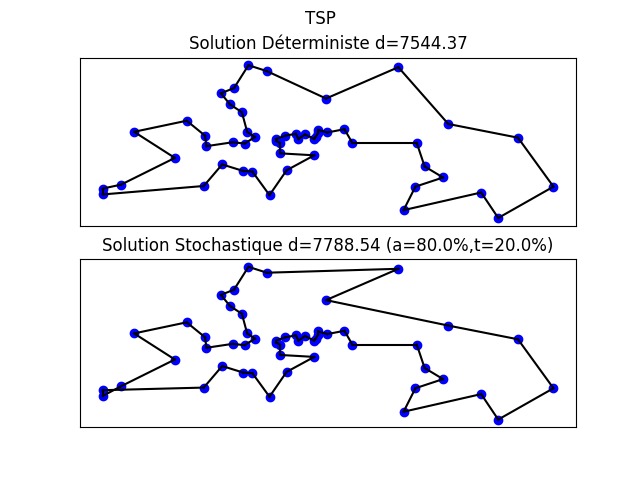
\includegraphics[width=0.5\textwidth]{g}}
\caption{Solution déterministe et stochastique pour le graphe berlin52.tsp}
\end{figure}\\
La distance théorique minimale obtenue est de 7544.37 (celle du problème déterministe). On peut voir, dans le problème stochastique, la solution optimale est à 7788.54, avec \(\alpha = 80\%\) et Z majorée de 20\%. Les chemins choisis sont différents dans les deux cas. Cela est du au fait que, en réalité, il existe des obstacles dans les chemins théoriques, le voyage doit donc prendre des autres chemins pour y arriver ainsi que pour obtenir son objectif.\\
\section{Recuit simulé pour le problème du voyageur de commerce}
On peut trouver de manière déterministe la meilleure solution à ce problème en explorant l’ensemble des solutions possibles, mais le coup du calcul devient vite pesant car celui-ci est de proportion factorielle (3.6 millions de possibilités pour 10 villes). Avec la méthode du recuit simulé, nous ne chercherons pas le meilleur trajet à coup sûr, mais nous chercherons à trouver un trajet optimal avec un coût bien moindre.\\
C’est un algorithme qui s’inspire de principes physiques. En effet, on a la montagne ci-dessous. On sait qu’un objet a toujours tendance à revenir à une position où l’énergie potentielle est minimum, autrement dit son altitude minimum ici le point rouge en bas à gauche. En physique, un système tend vers un état où l’énergie est le minimum possible. Cependant, si notre montagne possède des creux, l’objet initial au sommet de la montagne peut tomber dans un de ses creux qui ne sera pas l’altitude minimale globale mais locale, or on souhaite atteindre l’altitude minimale globale, là où l’énergie sera la plus faible.\\
 Cet algorithme s’inspire également de principes métallurgiques. Si on chauffe du métal, ce métal qui part d’un état initial va se déformer, recevoir de l’énergie et aura la forme de la montagne ci-dessous. Si on refroidit trop rapidement le métal, on peut se retrouver bloquer dans un des creux de la montagne, un état différent de l’état initial tandis que si on le refroidit très lentement, pour une température précise, on permet au métal d’atteindre l’équilibre thermique correspondant à l’état où l’énergie est minimale à cette température. Une fois atteint, on peut diminuer très lentement la température et on refait de même jusqu’à ce qu’on atteigne la température minimale. On aura à la fin un état optimal où l’énergie est la plus faible possible. (point rouge en bas à gauche de la montagne).\\
Le but de cet algorithme est donc d’atteindre un minimum qui n’est pas un minimum local (cuvette de la montagne) mais un minimum global (pied de la montagne).\\
\begin{figure}[h]\centering
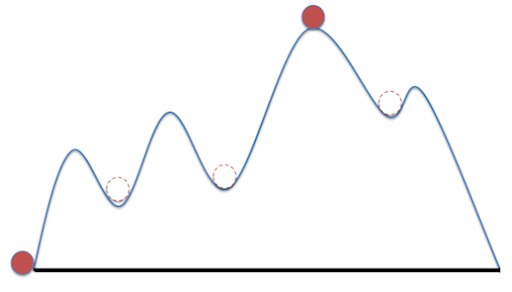
\includegraphics[width=0.5\textwidth]{rcd}
\caption{Le recuit simulé}
\end{figure}\\
Nous allons partir d’un point de départ (état) \(X_0\) correspondant à un trajet dont on va calculer la valeur de la solution (distance du trajet) et d’une température \(T_0\). Afin de trouver le minimum global, nous allons explorer le voisinage de \(X_0\) par le calcul des solutions des voisins de \(X_0\) que l’on nomme \(X_i\). (Ce voisinage correspond à modifier le trajet \(X_0\) en changeant l’ordre des villes où le voyageur passe).\\
Si l’état \(X_i\) permet de parcourir une distance plus faible que \(X_0\), on garde \(X_i\). Sinon, si \(X_i\) n’est pas mieux que \(X_0\), on calcule la différence entre la valeur des solutions de \(X_0\) et de \(X_i\) \(\Delta{E}\) . On tire entre 0 et 1 un nombre, si ce nombre est inférieur à \(e^{-dE/T}\)  (probabilité de Boltzmann), on garde \(X_i\) sinon on explore de nouveau le voisinage de \(X_i\).\\
On répète cela par cycle. A la fin du cycle, on applique une loi de décroissance de la température afin de calculer la nouvelle température. On vérifiera ensuite si l’on a atteint ou non la température minimale avant de recommencer le cycle. Notre algorithme sera terminé au moment où on aura atteint la température minimale que l’on a définie. Tant qu’on ne l’a pas atteint, on répète le cycle. 
\subsection{Réglages nécessaires pour l'algorithme du recuit simulé}
Afin de réaliser le recuit simulé pour notre problème du voyageur de commerce, il est nécessaire d’établir des paramètres qui seront essentiels à l’optimisation du trajet obtenu. 
\subsubsection{L'état initial}
En effet, en réalisant le recuit simulé pour ce problème, il est nécessaire de partir d’un état initial. Cet état initial \(X_0\) est donc un trajet que l’on a prédéfini en amont, ce trajet a donc une distance de parcours (notre solution E) dont on cherchera à la minimiser le plus possible en faisant le recuit simulé. On a décidé que l’état initial correspond au fait de parcourir les villes dans l’ordre (pour un graphe de n=10 villes, avec des villes qui sont numérotées de 0 à n - 1, le trajet sera: 0, 1, 2,…, 8, 9). Ce choix ne perturbera pas le fonctionnement de l’algorithme, il n’y a pas d’exigence requise sur la “qualité” de l’état initial. 
\subsubsection{La température}
Il faut considérer la température initiale \(T_0\) et la température minimale \(T_{min}\). Concernant la température initiale \(T_0\), il faut faire en sorte de bien la choisir. Elle doit être suffisamment haute pour assurer que l’équilibre thermique soit atteint rapidement. La température \(T_{min}\) impactera également la qualité de la solution si elle est trop élevée par exemple. Il faut tester et voir quelles sont les valeurs idéales pour notre algorithme que ce soit en termes de temps de calcul mais également en termes de qualité du résultat obtenu.
\subsubsection{Tau}
 Ce paramètre va impacter la vitesse à laquelle décroît notre température. Elle est contenue dans notre loi de décroissance de la température. Plus tau est élevé, plus la température va baisser lentement entre les cycles, d’où une décroissance plus lente de la température. Cela va impacter le temps de calcul ainsi que la qualité du résultat obtenu. 
\subsection{Choix des voisinages}
Pour exécuter l’algorithme du recuit simulé, il faut explorer le voisinage de \(X_i\). Cela revient à modifier le trajet de \(X_i\) pour obtenir \(X_{i+1}\), un état voisin de \(X_i\) ayant sa propre solution que l’on comparera à celle de \(X_i\). Dans notre code, on a voulu tirer de façon aléatoire deux numéros compris entre 0 et n-1 (avec n le nombre de villes dans notre graphe). Ces numéros correspondent à la position de la ville dans le trajet parcouru pour l’état \(X_i\). Si on a 5 villes et qu’on tire 0 et 3, cela correspond à la ville en position 0 (ville de départ) et la ville en position 3.  Dans cette intervalle en excluant la position 3 (entre position 0 et 2 inclus), on va modifier le trajet pour obtenir \(X_{i+1}\), un état voisin de \(X_i\). On va décaler les villes d’une position et la dernière ville de l’intervalle se retrouvera en 1ère position de l’intervalle. 
Par exemple, l’état \(X_i\) a pour trajet 1, 3, 4, 0, 2. Si on tire 0 et 3 , on s’occupe de la zone 1, 3, 4 et après modification, cela va donner 4,1,3. L’état \(X_{i+1}\) aura pour trajet 4, 1, 3, 0, 2.
\section{Recuit simulé stochastique}
TODO
\section{Conclusion}
TODO
\end{document}